\chapter{Background}
This chapter will give some background information to the key concepts that need to be understood
for this project. It will begin with a short introduction of ML and RL, how Deep Learning has
revolutionized the field, and a discussion on the current state of the art of DRL. The Q-Learning
algorithm will be explained in detail, as it is a prerequisite to understand the DRL algorithms Deep
Q-Learning, Double Q-Learning and Duel Q-Learning used in the implementation of this project.
Finally we will provide a discussion of the various tools and technologies that were considered for
use in the building of the system.

\section{Machine Learning}
% How machine learning is being used in games to learn -> Identify different approaches Focus in on
%   the RL approach -> What are the current approaches in RL -> Algorithms in use, tradeoffs NOT a
%   regurgitation of research papers -> Map out the current landscape in your own words What are the
%   key issues around RL -> In terms of performance -> What are the key metrics in use -> We then
%   use those metrics
\subsection{Introduction}
ML is a broad umbrella term for various methods of giving computer systems the ability to 'learn' to
complete some task efficiently using training and validation data, without being explicitly
programmed to do so. Instead of following a programmed set of instructions to make a prediction, the
ML system constructs a model that is a function approximated to some real world problem. ML tasks
can be divided into two categories; supervised and unsupervised learning. In supervised learning,
the dataset provides the correct output prediction, 'labelled' data, the system should make. The
system can use the input/output pairs to iteratively learn the best prediction, using a combination
of some generic error function, such as the \textit{Mean Squared Error}, and the \textit{Back
    Propagation} algorithm \cite{chauvin-bp} to update the model. In unsupervised learning, the dataset
does not contain any output data points, 'unlabelled' data, hence it is more difficult to gauge the
performance of an unsupervised ML algorithm. Unsupervised learning is generally used in the
clustering of data into classes. \paragraph{}

\subsection{Development of Machine Learning in Video Games}
In order to claim that an AI agent achieves general competency, it should be tested in a set of
environments that provide a suitable amount of variation, are reflective of real world problems the
agent might encounter, and that were created by an independent party to remove experimenter's bias
\cite{ale-eval-plat}. In this way, video games provide an effective test-bed for efficiently
studying general AI agents as they can provide all of these requirements. Although the application
of ML generated AI to video games may seem novel, the end goal is not to produce agents for
defeating world champion chess players, but to take these general agents and extend them to more
pressing problems to humanity, of which there are endless possibilities. \paragraph{}

The first application of notoriety to use computing to play a game arose in the research paper
``Programming a Computer for Playing Chess, 1950'' \cite{programming-comp-chess}, where
mathematician Claude Shannon developed an autonomous chess-playing system. In that paper, author
Shannon also highlighted the point that although the application of such a solution may seem
unimportant;
\begin{quote}
    ``It is hoped that a satisfactory solution of this problem will act as a wedge in attacking
    other problems of a similar nature and of greater significance''
\end{quote}
Claude designed a strategy that, even at the time, was infeasible as it would take more than 16
minutes to make a move. \paragraph{}

Fast forward to 1997, IBM developed ``Deep Blue,'' a network of computers purpose built to play
chess at an above-human level. It is renowned as the first AI system to defeat a world champion
chess player, Garry Kasparov under normal game regulations. There is an air of controversy
surrounding the feat, as IBM denied any chance of a replay after Kasparov claimed that IBM cheated
by actively programming moves into Deep Blue as the game was in play. \paragraph{}

In more recent times, British AI research company DeepMind published the paper ``Playing Atari with
Deep Reinforcement Learning, 2013'' \cite{deepmind1} in which they achieved far and above
human-level performance on a selection of 52 Atari2600 games with their Deep Q-Learning algorithm.
DeepMind have since applied their techniques to modern, real time, strategy game StarCraft2
\cite{starcraft}. This application was most impressive, as StarCraft2 is a game of imperfect
information. This means that not all aspects of the game are given to the player. In the context of
StarCraft2, the game map is not completely observable, the two players of the game cannot see what
the other is doing. All other exploits into the application of ML in video games up to then had been
on games of perfect information.

\section{Reinforcement Learning}
\subsection{Introduction}
RL is another case of ML tasks, which can come under the supervised and unsupervised learning
categories. It is a general way of approaching optimisation problems by trial and error. An agent
carries out actions in an environment, moving from one state to a new state and is given some
positive or negative numerical reward. This is known as the \textit{perception-action-learning
    loop}.

\begin{figure}[h]
    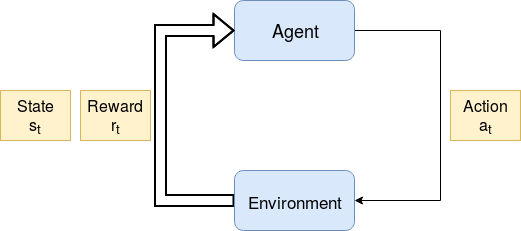
\includegraphics[scale=0.75]{rl_loop}
    \centering
    \caption{The perception-action-learning loop}
\end{figure}

RL is an interesting method of accomplishing ML tasks, as the agent can be given no prior
information about it's environment or the task, and it can learn based solely on trial and error,
reward and punishment. There are 3 main parts to a RL problem setup.

\begin{enumerate}
    \item An agent follows a \textit{policy} $\pi$, a rule that maps a state to an action.
    \item A \textit{reward function} $R(s, a)$, that gives an immediate value to an action $a$ taken
          by the agent to transition from state $s$ to $s'$
    \item A \textit{state value function} $V(s)$ that measures 'how good it is' to be in a given
          state. It assigns a value to the cumulate reward an agent can expect to gain by being in a
          state and following a policy through all subsequent states. We can define this as the
          \textit{discounted cumulative reward}:
          \begin{align*}
              V(s) = E(\sum_{t=0}\gamma^tR(s_t, a_t) | s_0 = s) \qquad \forall s \in S
          \end{align*}
\end{enumerate}

Where $\gamma$ is a discount factor $[0, 1]$ and we choose $a_t = \pi(s_t)$. The objective of a RL
problem is learning the optimal policy $\pi^*$, that for any given state will point the agent to the
most favourable action so as to maximize it's cumulative reward, $V^*(s) = \max_{\pi}V(s)$. RL
algorithms such as Q-Learning are used to find this optimal policy. \paragraph{}

\subsection{Markov Decision Process}
In a more formal setting, it is a soft assumption that RL problems qualify as a Markov Decision
Process (MDP) and can be modelled as such \cite{survey-drl}. MDP's display the Markov Property; that
the conditional probability distribution of future states is dependant only on the current state and
totally independent of all past states. A MDP consists of:

\begin{itemize}
    \item A finite set of states $S$
    \item A finite set of actions $A$
    \item A transition function $P(s, a, s') = P(s_{t+1}|s_t, a_t)$, a model mapping current state,
          action pairs to a probability distribution of potential future states.
    \item An immediate reward function $R(s, a)$
\end{itemize}

Again, an MDP seeks to find the optimal policy $\pi^*$. We define $\pi^*$ as

\begin{align*}
    \pi^* = argmax_a\{\sum_{s'}P(s, a, s')(R(s, a) + \gamma V(s')\}
\end{align*}

\subsection{Model-Free Learning}
Not all RL problems are provided with a transition function $P(s, a, s')$. In fact, it is more often
than not that we cannot express the agent's environment with a model. Such a scenario is called
\textit{model-free learning}, where the agent must learn the optimal policy without the use of a
transition function to guide it on which action to take. Instead it must devise some other way of
modelling it's environment, such as building a 'memory' of actions and rewards based on experiences
and deriving an optimal policy from these experiences. The downside to this is the potentially large
amounts of auxiliary space needed to store the experiences. This is where algorithms such as
Q-Learning are used. \paragraph{}

Q-Learning is a model free RL algorithm. At each state, the agent calculates an immediate reward,
based solely on the current state and action taken, and the \textit{quality} of taking an action $a$
in state $s$ and following a policy $\pi$ thereafter, called the Q-Value, which is defined as:

\begin{gather*}
    Q(s, a) = E(\sum_{t=0}\gamma^tR(s_t, a_t) | s_0 = s, a_0 = a) \qquad \forall s \in S
\end{gather*}

Where we have chosen $a_0$ arbitrarily and
choose all subsequent $a_t = \pi(s_t)$ thereafter. As the agent explores all states multiple times
and experiments with different actions, the corresponding Q-values are saved and updated in a data
structure, hence an optimum policy can be derived by finding the optimum Q-values $Q^*(s, a)$ for all states after a predetermined number of iterations or until the policy is 'good enough'. The update step for a Q-Value is defined as:

\begin{align*}
    Q(s_t, a_t) \leftarrow (1-\alpha)Q(s_t, a_t) + \alpha(r_t + \gamma max_aQ(s_{t+1}, a))
\end{align*}

Where $\alpha$ is a hyperparameter called the \textit{learning rate} chosen in the range $(0, 1)$. As $t \rightarrow \infty, Q_t \rightarrow Q^*_t$, we converge on an optimum solution. The data structure used to store the agent's experiences can be referred to as the Q-Matrix. It is a
$|S| x |A|$ sized matrix, that is the total number of states x total number of available actions.

\begin{figure}[h]
    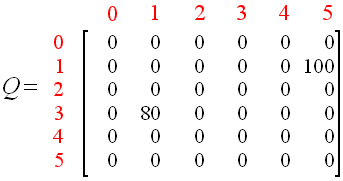
\includegraphics[scale=0.75]{q_matrix}
    \centering
    \caption{An example Q-Matrix. 0 indicates an unexplored state, action pair}
\end{figure}

The agent follows the algorithm \ref{alg:QL}, detailed below.
After a suitable number of iterations and exploration, the Q-Matrix becomes a 'map' for the agent,
whereby it can look up the action with the highest Q-Value for any state \cite{qlearning}.
Q-Learning is a straight-forward, elegant solution to a RL task. However, for an environment space
of high dimensionality, such as an array of RGB pixels from an image, the Q-Matrix becomes
infeasibly large in the $S$ dimension and increasingly sparse, as only a small percentage of the
total available state, action pairs will be visited. As a worked example, imagine a robot that is
using Q-Learning to find a path from it's current position to some exit room. If the robot takes
210x160, 8-bit colour space, RGB photos of it's surroundings to represent a state, the $S$ dimension
becomes $256^{210x160x3}$ in size. A solution to the dimensionality problem was
proposed by DeepMind, in the paper ``Playing Atari with Deep Reinforcement Learning, 2013''
\cite{deepmind1} which will be discussed later in this chapter.

\begin{algorithm}
    \caption{Q-Learning Algorithm}\label{alg:QL}
    \begin{algorithmic}[1]
        \Procedure{Building Q-Matrix}{}
        \State Set $\alpha$ and $\gamma$ parameters.
        \State Initialize Q-Matrix to zero.
        \Repeat
        \While{Goal/terminal state not reached}
        \State Select $a$ randomly from all possible actions in current state
        \State Consider going to state $s_{t+1}$ from state $s$ using action $a$
        \State Get maximum Q-Value from $s_{t+1}$ considering all possible actions
        \State $Q(s, a) \gets (1-\alpha)Q(s_t, a_t) + \alpha(r_t + \gamma max_aQ(s_{t+1}, a))$
        \EndWhile
        \Until{Policy good enough}
        \EndProcedure
        \Procedure{Using Q-matrix}{}
        \State $s \gets$ initial state
        \While{Goal/terminal state not reached}
        \State $a \gets max_{a}Q(s, a)$
        \State $s \gets s_{t+1}$ taking action $a$
        \EndWhile
        \EndProcedure
    \end{algorithmic}
\end{algorithm}

\subsection{Exploration vs. Exploitation}
There is a fundamental issue in any RL task, where the agent must choose between taking an
instantaneous reward by exploiting the policy, or taking a random action to explore the environment
in search of a potentially higher long term reward. This problem is illustrated by a well-known RL
problem known as the k-armed bandit problem.

\begin{quotation}
    ``The agent is in a room with a collection of $k$ gambling machines (each called a `one armed
    bandit' in colloquial English). The agent is permitted a fixed number of pulls, $h$. Any arm may
    be pulled on each turn. The machines do not require a deposit to play; the only cost is in
    wasting a pull playing a suboptimal machine. When arm $i$ is pulled, machine $i$ pays off 1 or
    0, according to some underlying probability parameter $p_i$, where payoffs are independent
    events and the $p_i$'s are unknown. What should the agent's strategy be?''
    \cite{kaelbling1996reinforcement}
\end{quotation}

The amount of time the agent spends in the environment is one factor that can be taken into
consideration when making this decision. In general, the longer the agent spends in the environment,
the less impact taking an exploratory approach, sometimes towards a sub-optimal policy, will have on
the end policy. \paragraph{}

One solution to this dilemma is to take an \textit{epsilon greedy policy}. At each state, the agent
takes a random action with a probability of $\epsilon$ and an action from the policy with a
probability of $(1-\epsilon)$. $\epsilon$ is linearly reduced at each iteration to some
predetermined floor value. This way, the agent will spend more time exploring at the start of it's
interaction with the environment, and will then (hopefully) converge to an optimal policy as it progresses.

\subsection{Deep Reinforcement Learning}
DRL refers to the use of deep learning algorithms within the field of RL. As mentioned previously, RL struggles with environments of high dimensionality. DRL overcomes this issue thanks to the universal function approximation property of deep neural networks and their abilities to isolate and recognize features of interest within high dimensional data and to compactly represent that high dimensional input data \cite{survey-drl}. DRL can utilize a convolutional neural network to learn a representation of the environment on behalf of the agent through high dimensional sensory input such as video data. A set of fully connected layers are then generally used to approximate the target of the underlying RL algorithm, such as $V(s, a)$, $Q(s, a)$, an action etc. The deep neural network can then be trained using an appropriate variant of the backpropagation algorithm, such as stochastic or batch gradient descent. \paragraph{}

The event that brought DRL to the attention of the research community was from the paper mentioned earlier ``Playing Atari with Deep Reinforcement Learning, 2013''. DeepMind created a variant of Q-Learning called Deep Q-Learning (DQL), that achieved above-human level performance on a large selection of 52 Atari 2600 video games. They combined a convolutional neural network for feature detection, and a fully connected network to learn the Q-Values for all available actions, with ReLU activations between each layer. The network uses a standard Least Square Error loss function in training with gradient Propagation, defined as:

\begin{align*}
    L = (y_i - Q(s, a))^2 \\
    y_i = r + \gamma max_{a^*}Q(s', a^*)
\end{align*}

This architecture was named the Deep Q-network. This breakthrough successfully removes the dimensionality problem, as there is no need to keep a data structure storing all previous experiences. The deep neural network takes an array of RGB pixel information, taken as a stack of 3/4 (depending on the game) greyscale frames, as input to the convolutional network. The fully connected network outputs a vector of Q-Values for each available action in the game. \paragraph{}

\begin{figure}[H]
    \centering
    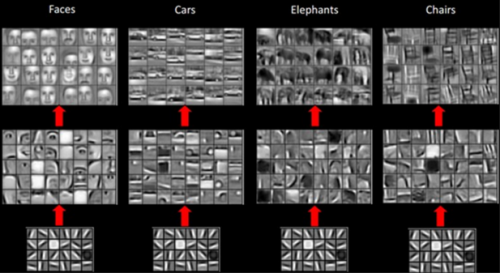
\includegraphics[scale=0.6]{conv_filter}
    \caption{Examples of output filters from a convolution neural network}
\end{figure}
\begin{figure}[H]
    \centering
    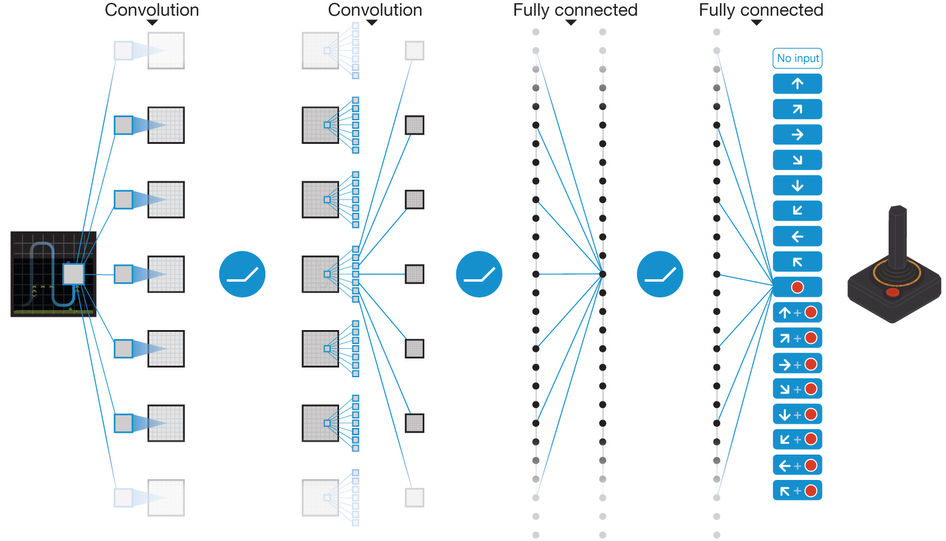
\includegraphics[scale=0.4]{dqn_arch}
    \caption{The original Deep Q-network Architecture}
\end{figure}

At the time, this breakthrough was the state of the art. Since then, many improvements and adaptations have been made on this model, by DeepMind and other research groups. Such examples include the Double Q-Learning adaptation \cite{doubleq} and the Dueling Q-network architecture \cite{dueling}. Experience replay and target networks were two techniques added to the original architecture by DeepMind to provide more stability to the learning process. \paragraph{}

Instead of learning from the immediately previous experience when training the network, a large memory of past experiences are stored as tuples of $(s_t, a_t, r_{t}, s_{t+1}, term)$, where $term$ is a boolean indicating if this state transition was terminal (a gameover). The network is then trained from a random sampling of past experiences from this replay memory. It was found to greatly reduce the number of interactions the agent needed to have with the environment. However, this technique \textit{is somewhat} limited as there is no way to differentiate important experiences from unimportant ones. In the State of the Art section we will discuss an optimization to experience replay that mitigates this drawback \cite{human}. \paragraph{}

The target network is a secondary network $\hat{Q}$ cloned from the original Q-network $Q$, that is used to predict the targets $y_i$ when training $Q$. The weights of $\hat{Q}$ are cloned from $Q$ every $C$ training steps. This modification makes the algorithm more stable, as an increase to $Q(s_t, a_t)$ was often found to also increase $Q(s_{t+1}, a)$ for all $a$, thus also increasing the targets $y_i$. This can create a diverging solution in some cases. Freezing the weights makes the updates to $Q$ and the targets $y$ further apart, decreasing the likelihood of divergence \cite{human}. \paragraph{}

\begin{algorithm}
    \caption{Deep Q-Learning Algorithm with Experience Replay}\label{alg:QN}
    \begin{algorithmic}[1]
        \State Initialize replay memory $D$ to capacity $N$
        \State Initialize $Q$ with random weights $\theta$
        \For{episode = 1, M}
        \State Initialize arbitrary first sequence of states
        \For{t = 1, T}
        \State With probability $\epsilon$ select a random action $a_t$, otherwise select $a_t = max_a Q(s_t, a)$
        \State Execute action $a_t$ and observe reward $r_t$ and state $s_{t+1}$
        \State Store state transition $(s_t, a_t, r_t, s_{t+1}, term)$ in $D$
        \State Sample random mini batch $(s_i, a_i, r_i, s_{i + 1}, term)$ from $D$
        \If{$term = true$}
        \State Set $y_i = r_i$
        \Else
        \State Set $y_i = \gamma max_a Q(s_{i+1}, a)$
        \EndIf
        \EndFor
        \State Perform a gradient descent step on $(y_i - Q(s_i, a_i))^2$
        \EndFor
    \end{algorithmic}
\end{algorithm}

The applications have been broadened to fields such as natural language processing and robotics. More detail on the current state of the art will be given in the next section.

\section{State of the Art}
The current state of the field of RL is vast. More and more it is being utilized as the next step towards more efficient and intelligent ML systems \cite{survey-drl}. This section will be divided into two discussions. The first will give a broad, relatively brief overview of the types of applications of RL today. The second section will discuss the state of the art for RL research with the video game test bed. This will primarily focus on the work of DeepMind, as their work is most pertinent to this project. 
